\documentclass[10pt]{article}
\usepackage{amsmath}
\usepackage{tikz}
\usepackage{amsfonts}
\usepackage{enumitem}
\usepackage[math-style=ISO,bold-style=ISO,mathrm=sym]{unicode-math}
\usepackage{pdfpages}
\usepackage{tikz}
\usepackage{xcolor}
\usepackage{xfp}
\usepackage[top=5mm, bottom=2mm, inner=5mm, outer=5mm,
headheight=0mm, headsep=0mm, footskip=0mm,
papersize={210mm, 148mm},
includeheadfoot
]{geometry}
\newcommand{\heading}[1]{
\begin{center}
\setmainfont{Raleway SemiBold}[Scale=1.3]#1
\end{center}\vspace{-7mm}}
\newcommand{\subheading}[1]{
\vspace{-2mm}
\begin{flushleft}
\setmainfont{Raleway SemiBold}[Scale=1]#1
\end{flushleft}\vspace{-5mm}}

\defaultfontfeatures{Ligatures=TeX}
\setmainfont[BoldItalicFont=Linux Biolinum Slanted Bold]{Libertinus Sans}
\setmathfont[NFSSFamily=mathfont,RawFeature={+ss08}]{Libertinus Math}
\DeclareMathAlphabet{\mathcal}{OMS}{cmsy}{m}{n}

% Replace 0-9 with sans serif versions
%\DeclareSymbolFont{MathFont}{TU}{mathfont}{m}{n}
\Umathcode "31 = "0"0"1D7E3
\Umathcode "32 = "0"0"1D7E4
\Umathcode "33 = "0"0"1D7E5
\Umathcode "34 = "0"0"1D7E6
\Umathcode "35 = "0"0"1D7E7
\Umathcode "36 = "0"0"1D7E8
\Umathcode "37 = "0"0"1D7E9
\Umathcode "38 = "0"0"1D7EA
\Umathcode "39 = "0"0"1D7EB
\Umathcode "30 = "0"0"1D7E2


\pagestyle{empty}

\newenvironment{enumerlist}[1][5mm]{\begin{enumerate}[leftmargin=#1]
  \setlength{\itemsep}{1pt}
  \setlength{\parskip}{0pt}
}{\end{enumerate}}
\begin{document}
\noindent\begin{minipage}[t][138mm][t]{95mm}
\heading{Definitions}
\vspace{3mm}
{\footnotesize
\begin{enumerlist}[0mm]
\item[] The \textbf{integers} are the numbers \dots, $-3$, $-2$, $-1$, $0$, $1$, $2$, $3$, \dots
\item[] The \textbf{positive integers} are the numbers 1, 2, 3, \dots
\end{enumerlist}
}

\vspace{2mm}

\heading{Hints}
\vspace{3mm}
{\footnotesize
\begin{enumerlist}[10mm]
\item[1.] There are only a few odd numbers to add up.
\item[2.] What is the sum of the odd integers between 0 and 2? Between 0 and 4? 0 and 6? What's the pattern?
\item[3.] Try some numbers of baubles between 2 and 20.
\item[4.] What would be the answer for 2 or 3 people? Or 2 or 3 or 4 people? Can you generalise?
\item[5.] It's not too much bigger than 100.
\item[6.] How many one-digit integers? How many two-digit integers? How many three-digit integers? {\dots} What's the most digits the number could have?
\item[7.] If you find four numbers in a row that you can make, you could make all larger scores by adding some 4s.
\item[8.] Try it with a few smaller numbers and look for a pattern.
\item[9.] $10=1+2+3+4$, $11=5+6$, $12=3+4+5$. Keep going until there's one you can't do.
\item[10.] What's special about numbers that are the sum of four consecutive integers?
\item[11.] Try it with 3 points, 4 points, 5 points, and look for a pattern.
\item[12.] Use your pattern from 11.
\end{enumerlist}
}

%\heading{Solutions}
%\vspace{3mm}
%{\footnotesize
%
%}
\vfill
\begin{center}\footnotesize
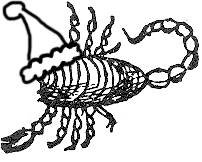
\includegraphics[width=.14\textwidth]{scorpion.png}
\\

\includegraphics[width=.75\textwidth]{logo.jpg}
\\
\begin{minipage}{3.5cm}
chalkdustmagazine.com
\\
@chalkdustmag
\\
\#ChalkdustChristmasCard2026
\end{minipage}
\end{center}
\end{minipage}\hspace{10mm}\begin{minipage}[t][138mm][t]{95mm}
\vspace*{3mm}

\begin{center}
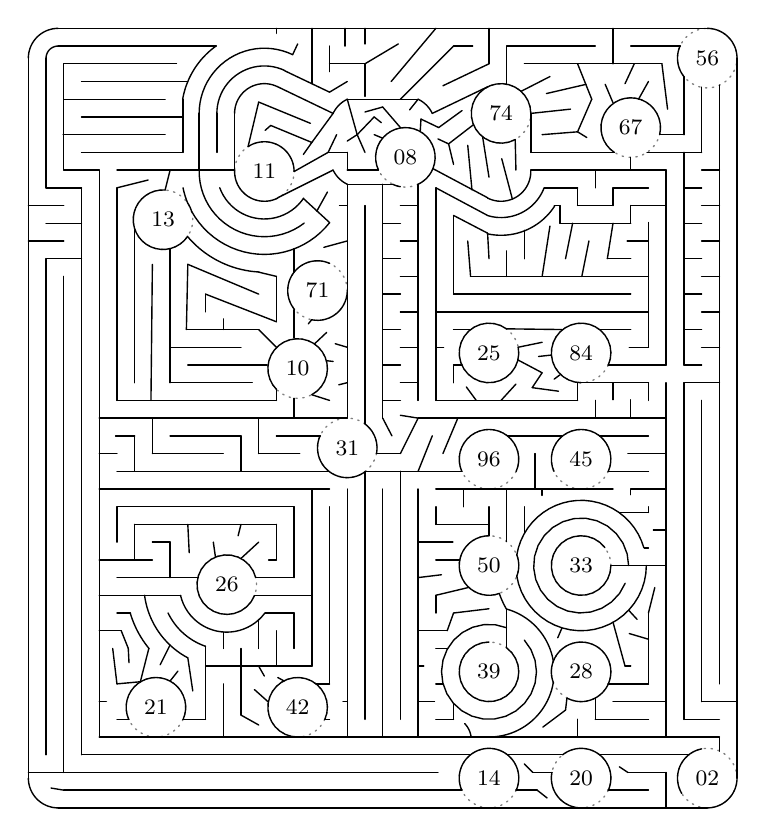
\begin{tikzpicture}[y=9mm,x=9mm,line width=0.5pt,line cap=round,line join=round]
\footnotesize

\foreach \x/\y in {0.32/4.18,-1.67/3.98,1.67/4.8,-0.5/0.08,2.8/-0.08,1.5/-0.08,1.5/1.42,2.8/1.42,1.5/-1.58,2.8/-1.58,1.5/-3.08,2.8/-3.08,-1.2/1.2,-0.92/2.3,-3.1/3.3,-3.2/-3.58,-2.2/-1.848,-1.2/-3.58,1.5/-4.58,2.8/-4.58,3.5/4.6,4.58/5.58,4.58/-4.58}
    \draw[gray,dotted] (\x,\y) circle (0.42);

\draw (3.18,-0.25) -- (3.75,-0.25);
\draw (3.46,0) -- (4,0);
\draw (3.06,0.25) -- (3.75,0.25);
\draw (4,0.5) -- (0.5,0.5);
\draw (2.53,0.25) -- (1.76,0.25);
\draw (2.15,0) -- (2.15,-0.5);
\draw (0.25,-0.5) -- (0.25,-3.75);
\draw (0,-0.5) -- (0,-4);
\draw (-0.25,-3.75) -- (-0.25,-0.5);
\draw (-0.5,-4) -- (-0.5,-0.5);
\draw (0.5,-4) -- (-0.5,-4);
\draw (0.5,-4) -- (0.5,-0.5);
\draw (-4,-0.5) -- (-4,0.5);
\draw (-4,0.5) -- (-0.5,0.5);
\draw (-3.5,-0.25) -- (-3.5,0.25);
\draw (-3.5,0.25) -- (-3.77,0.25);
\draw (-4,0) -- (-3.75,0);
\draw (-3.25,0.5) -- (-3.25,0);
\draw (-2.25,0) -- (-3.25,0);
\draw (-2,-0.25) -- (-2,0.25);
\draw (-2,0.25) -- (-3,0.25);
\draw (-1.75,0.5) -- (-1.75,0);
\draw (4,0.5) -- (4,-0.5);
\draw (0.25,-0.5) -- (0.25,-0.25);
\draw (1.12,-0.25) -- (0.25,-0.25);
\draw (3.22,-1.58) -- (3.72,-1.58);
\draw (3.75,-1.33) -- (3.69,-1.33);
\draw (4,-1.08) -- (3.82,-1.08);
\draw (3.33,-0.83) -- (3.75,-0.83);
\draw (3.75,-0.83) -- (3.75,-0.75);
\draw (3.5,-0.58) -- (3.5,-0.5);
\draw (4,-1.58) -- (3.72,-1.58);
\draw (4,-1.58) -- (4,-4);
\draw (4,-4) -- (0.5,-4);
\draw (2.25,-0.5) -- (2.25,-0.59);
\draw (2,-1.13) -- (2,-0.75);
\draw (1.75,-1.24) -- (1.75,-0.5);
\draw (1.75,-2.74) -- (1.75,-2.19);
\draw (1,-3.53) -- (1,-3.75);
\draw (1,-3.75) -- (0.75,-3.75);
\draw (0.73,-3.5) -- (0.5,-3.5);
\draw (0.85,-3.25) -- (0.75,-3.25);
\draw (0.58,-3) -- (0.5,-3);
\draw (0.92,-2.75) -- (0.75,-2.75);
\draw (0.91,-2.5) -- (0.5,-2.5);
\draw (1.5,-1.16) -- (1.5,-0.75);
\draw (0.91,-2.5) -- (1,-2.25);
\draw (1,-2.25) -- (1.5,-2.19);
\draw (1.21,-1.89) -- (0.75,-2);
\draw (0.75,-2.25) -- (0.75,-2);
\draw (0.5,-1.75) -- (0.83,-1.71);
\draw (0.75,-1.5) -- (1.09,-1.5);
\draw (0.99,-1.25) -- (0.5,-1.25);
\draw (1.5,-1) -- (0.75,-1);
\draw (0.75,-1) -- (0.75,-0.75);
\draw (1.14,-0.5) -- (1.14,-0.75);
\draw (2.26,-3.86) -- (2.58,-3.62);
\draw (2.58,-3.62) -- (2.6,-3.45);
\draw (2.75,-3.75) -- (2.75,-4);
\draw (3,-3.45) -- (3,-3.75);
\draw (3,-3.75) -- (3.75,-3.75);
\draw (4,-3.5) -- (3.25,-3.5);
\draw (3.18,-3.25) -- (3.75,-3.25);
\draw (3.75,-3.25) -- (3.75,-2.25);
\draw (3.75,-2.25) -- (3.84,-1.89);
\draw (2.53,-2.46) -- (2.47,-2.6);
\draw (3.25,-2.38) -- (3.42,-3);
\draw (3.42,-3) -- (3.5,-3);
\draw (3.75,-2.62) -- (3.48,-2.54);
\draw (3.47,-2.21) -- (3.59,-2.34);
\draw (0.75,-0.5) -- (3.25,-0.5);
\draw (3.5,-0.5) -- (4,-0.5);
\draw (4,-1.58) -- (4,-0.5);
\draw (3.18,1.25) -- (4,1.25);
\draw (4,1.25) -- (4,4);
\draw (2.8,1) -- (3.75,1);
\draw (4,1) -- (4,0.5);
\draw (3.75,1) -- (3.75,0.75);
\draw (3.5,0.5) -- (3.5,0.76);
\draw (3.25,0.99) -- (3.25,0.76);
\draw (3,0.5) -- (3,0.75);
\draw (2.75,1) -- (2.75,0.75);
\draw (2.75,0.75) -- (0.75,0.75);
\draw (0.5,0.75) -- (0.5,3.8);
\draw (0.75,0.75) -- (0.75,3.75);
\draw (0.71,4.02) -- (1.48,3.61);
\draw (0.75,3.75) -- (1.48,3.36);
\draw (2.28,3.75) -- (2.75,3.75);
\draw (2.75,3.75) -- (2.75,3.5);
\draw (2.75,3.5) -- (3.25,3.5);
\draw (3.25,3.5) -- (3.25,3.75);
\draw (3.25,3.75) -- (3.75,3.75);
\draw (4,3.5) -- (3.5,3.5);
\draw (3,4) -- (3,3.75);
\draw (4,4) -- (2.09,4);
\draw (3.5,3.5) -- (3.5,3.25);
\draw (1,3.36) -- (1.48,3.11);
\draw (2.42,3.5) -- (2.5,3.5);
\draw (3.5,3.25) -- (2.5,3.25);
\draw (2.5,3.25) -- (2.5,3.5);
\draw (3.75,3.26) -- (3.75,1.5);
\draw (3.75,1.5) -- (3.48,1.5);
\draw (3.06,1.75) -- (3.5,1.75);
\draw (3.75,2) -- (0.75,2);
\draw (2.53,1.75) -- (1.75,1.76);
\draw (1.24,1.75) -- (1,1.75);
\draw (0.75,1.5) -- (0.86,1.5);
\draw (1.12,1.25) -- (1,1.25);
\draw (1,1.25) -- (1,1);
\draw (1.32,0.75) -- (1.18,0.94);
\draw (1.67,0.75) -- (1.88,0.98);
\draw (1.91,1.32) -- (2.25,1.14);
\draw (2.25,1.14) -- (2.11,0.93);
\draw (2.11,0.93) -- (2.48,0.88);
\draw (2.5,1.11) -- (2.42,1.05);
\draw (1.91,1.5) -- (2.25,1.57);
\draw (2.38,1.39) -- (2.2,1.37);
\draw (1,3.36) -- (1,2.25);
\draw (1,2.25) -- (3.5,2.25);
\draw (3.75,2.5) -- (1.24,2.5);
\draw (1.24,2.5) -- (1.2,3);
\draw (1.48,3.11) -- (1.5,2.75);
\draw (1.75,2.5) -- (1.75,2.86);
\draw (2,3.15) -- (2,2.75);
\draw (2.25,2.5) -- (2.36,3.21);
\draw (2.68,3.25) -- (2.58,2.75);
\draw (2.81,2.5) -- (2.91,3);
\draw (3.25,3.25) -- (3.17,2.75);
\draw (3.17,2.75) -- (3.5,2.75);
\draw (3.75,3) -- (3.45,3);
\draw (1.06,0.5) -- (0.85,0);
\draw (0.5,-0.25) -- (0.7,0.25);
\draw (0.5,0.5) -- (0.25,0);
\draw (-0.5,0.5) -- (-0.5,3.8);
\draw (-0.25,0.42) -- (-0.25,3.5);
\draw (-0.5,3.8) -- (0,3.8);
\draw (0,3.8) -- (0,0.5);
\draw (0,0.5) -- (0.13,0.25);
\draw (0.5,0.5) -- (0.25,0.54);
\draw (0,0.75) -- (0.25,0.75);
\draw (0.5,1) -- (0.25,1);
\draw (0,1.25) -- (0.25,1.25);
\draw (0.5,1.5) -- (0.25,1.5);
\draw (0,1.75) -- (0.25,1.75);
\draw (0.5,2) -- (0.25,2);
\draw (0,2.25) -- (0.25,2.25);
\draw (0.5,2.5) -- (0.25,2.5);
\draw (0,2.75) -- (0.25,2.75);
\draw (0.5,3) -- (0.25,3);
\draw (0,3.25) -- (0.25,3.25);
\draw (0.5,3.5) -- (0.25,3.5);
\draw (0,3.8) -- (0.14,3.8);
\draw [shift={(2.8,-0.08)}] plot[domain=-0.42:3.56,variable=\t]({1*0.42*cos(\t r)+0*0.42*sin(\t r)},{0*0.42*cos(\t r)+1*0.42*sin(\t r)});
\draw [shift={(-0.32,4.18)}] plot[domain=3.58:4.27,variable=\t]({1*0.42*cos(\t r)+0*0.42*sin(\t r)},{0*0.42*cos(\t r)+1*0.42*sin(\t r)});
\draw [shift={(1.5,-0.08)}] plot[domain=-0.42:3.56,variable=\t]({1*0.42*cos(\t r)+0*0.42*sin(\t r)},{0*0.42*cos(\t r)+1*0.42*sin(\t r)});
\draw [shift={(2.8,-1.58)}] plot[domain=-5.64:0,variable=\t]({1*0.42*cos(\t r)+0*0.42*sin(\t r)},{0*0.42*cos(\t r)+1*0.42*sin(\t r)});
\draw [shift={(2.8,-1.58)}] plot[domain=0:5.9,variable=\t]({1*0.67*cos(\t r)+0*0.67*sin(\t r)},{0*0.67*cos(\t r)+1*0.67*sin(\t r)});
\draw [shift={(2.8,-1.58)}] plot[domain=0.28:2.98,variable=\t]({1*0.92*cos(\t r)+0*0.92*sin(\t r)},{0*0.92*cos(\t r)+1*0.92*sin(\t r)});
\draw [shift={(2.8,-1.58)}] plot[domain=-2.98:0,variable=\t]({1*0.92*cos(\t r)+0*0.92*sin(\t r)},{0*0.92*cos(\t r)+1*0.92*sin(\t r)});
\draw [shift={(1.5,-1.58)}] plot[domain=-0.37:0.37,variable=\t]({1*0.42*cos(\t r)+0*0.42*sin(\t r)},{0*0.42*cos(\t r)+1*0.42*sin(\t r)});
\draw [shift={(1.5,-3.08)}] plot[domain=-4.71:0.93,variable=\t]({1*0.42*cos(\t r)+0*0.42*sin(\t r)},{0*0.42*cos(\t r)+1*0.42*sin(\t r)});
\draw [shift={(1.5,-3.08)}] plot[domain=-5.09:0.73,variable=\t]({1*0.67*cos(\t r)+0*0.67*sin(\t r)},{0*0.67*cos(\t r)+1*0.67*sin(\t r)});
\draw [shift={(1.5,-3.08)}] plot[domain=0.16:1.3,variable=\t]({1*0.92*cos(\t r)+0*0.92*sin(\t r)},{0*0.92*cos(\t r)+1*0.92*sin(\t r)});
\draw [shift={(1.5,-3.08)}] plot[domain=4.71:6.12,variable=\t]({1*0.92*cos(\t r)+0*0.92*sin(\t r)},{0*0.92*cos(\t r)+1*0.92*sin(\t r)});
\draw [shift={(2.8,-3.08)}] plot[domain=2.78:3.51,variable=\t]({1*0.42*cos(\t r)+0*0.42*sin(\t r)},{0*0.42*cos(\t r)+1*0.42*sin(\t r)});
\draw [shift={(0.92,-4.04)}] plot[domain=0.14:0.77,variable=\t]({1*0.33*cos(\t r)+0*0.33*sin(\t r)},{0*0.33*cos(\t r)+1*0.33*sin(\t r)});
\draw [shift={(2.8,-1.58)}] plot[domain=3.47:3.67,variable=\t]({1*1.22*cos(\t r)+0*1.22*sin(\t r)},{0*1.22*cos(\t r)+1*1.22*sin(\t r)});
\draw [shift={(1.5,-1.58)}] plot[domain=1.57:5.07,variable=\t]({1*0.42*cos(\t r)+0*0.42*sin(\t r)},{0*0.42*cos(\t r)+1*0.42*sin(\t r)});
\draw [shift={(2.8,-3.08)}] plot[domain=-0.42:2.78,variable=\t]({1*0.42*cos(\t r)+0*0.42*sin(\t r)},{0*0.42*cos(\t r)+1*0.42*sin(\t r)});
\draw [shift={(2.8,-3.08)}] plot[domain=4.23:5.21,variable=\t]({1*0.42*cos(\t r)+0*0.42*sin(\t r)},{0*0.42*cos(\t r)+1*0.42*sin(\t r)});
\draw [shift={(2.8,1.42)}] plot[domain=-0.42:4.71,variable=\t]({1*0.42*cos(\t r)+0*0.42*sin(\t r)},{0*0.42*cos(\t r)+1*0.42*sin(\t r)});
\draw [shift={(0.32,4.18)}] plot[domain=5.16:5.9,variable=\t]({1*0.42*cos(\t r)+0*0.42*sin(\t r)},{0*0.42*cos(\t r)+1*0.42*sin(\t r)});
\draw [shift={(1.67,3.98)}] plot[domain=4.42:5.92,variable=\t]({1*0.65*cos(\t r)+0*0.65*sin(\t r)},{0*0.65*cos(\t r)+1*0.65*sin(\t r)});
\draw [shift={(1.67,3.98)}] plot[domain=4.5:5.71,variable=\t]({1*0.9*cos(\t r)+0*0.9*sin(\t r)},{0*0.9*cos(\t r)+1*0.9*sin(\t r)});
\draw [shift={(1.5,1.42)}] plot[domain=-5.35:0.19,variable=\t]({1*0.42*cos(\t r)+0*0.42*sin(\t r)},{0*0.42*cos(\t r)+1*0.42*sin(\t r)});
\draw [shift={(1.67,3.98)}] plot[domain=-2.04:0.05,variable=\t]({1*0.42*cos(\t r)+0*0.42*sin(\t r)},{0*0.42*cos(\t r)+1*0.42*sin(\t r)});
\draw [shift={(0.32,4.18)}] plot[domain=4.27:4.54,variable=\t]({1*0.42*cos(\t r)+0*0.42*sin(\t r)},{0*0.42*cos(\t r)+1*0.42*sin(\t r)});
\draw [shift={(0.32,4.18)}] plot[domain=-0.38:3.58,variable=\t]({1*0.42*cos(\t r)+0*0.42*sin(\t r)},{0*0.42*cos(\t r)+1*0.42*sin(\t r)});
\draw (-0.06,4) -- (-0.5,4);
\draw (-0.5,4) -- (-0.5,4.25);
\draw (-0.77,4.25) -- (-1.25,3.98);
\draw (-0.7,4) -- (-1.48,3.61);

\draw [shift={(-1.67,3.98)}] plot[domain=0:2.15,variable=\t]({1*0.42*cos(\t r)+0*0.42*sin(\t r)},{0*0.42*cos(\t r)+1*0.42*sin(\t r)});
\draw [shift={(-1.67,3.98)}] plot[domain=3.09:5.18,variable=\t]({1*0.42*cos(\t r)+0*0.42*sin(\t r)},{0*0.42*cos(\t r)+1*0.42*sin(\t r)});
\draw [shift={(-1.67,3.98)}] plot[domain=3.49:5.69,variable=\t]({1*0.67*cos(\t r)+0*0.67*sin(\t r)},{0*0.67*cos(\t r)+1*0.67*sin(\t r)});
\draw [shift={(-1.67,3.98)}] plot[domain=3.12:5.37,variable=\t]({1*0.92*cos(\t r)+0*0.92*sin(\t r)},{0*0.92*cos(\t r)+1*0.92*sin(\t r)});
\draw [shift={(-1.67,3.98)}] plot[domain=3.34:3.53,variable=\t]({1*1.17*cos(\t r)+0*1.17*sin(\t r)},{0*1.17*cos(\t r)+1*1.17*sin(\t r)});
\draw [shift={(-1.67,3.98)}] plot[domain=3.64:5.62,variable=\t]({1*1.17*cos(\t r)+0*1.17*sin(\t r)},{0*1.17*cos(\t r)+1*1.17*sin(\t r)});
\draw [shift={(-1.67,3.98)}] plot[domain=3.84:4.66,variable=\t]({1*1.42*cos(\t r)+0*1.42*sin(\t r)},{0*1.42*cos(\t r)+1*1.42*sin(\t r)});

\draw (-2.09,4) -- (-2.09,4.8);
\draw [shift={(-1.67,4.8)}] plot[domain=1.12:pi,variable=\t]({1*0.42*cos(\t r)+0*0.42*sin(\t r)},{0*0.42*cos(\t r)+1*0.42*sin(\t r)});
\draw (-1.49,5.18) -- (-0.7,4.8);
\draw (-0.77,4.25) -- (-0.5,4.25);
\draw (-1.9,4.33) -- (-1.75,4.96);
\draw (-1.75,4.96) -- (-1.02,4.66);
\draw (-0.7,4.8) -- (-1,4.39);
\draw (-1,4.39) -- (-1.58,4.63);
\draw (-1.58,4.63) -- (-1.66,4.56);
\draw (-1,4.39) -- (-1.12,4.22);
\draw (-0.77,4.25) -- (-0.65,4.5);
\draw (-0.5,5) -- (-0.36,4.5);
\draw (-0.36,4.5) -- (-0.5,4.41);
\draw (-0.36,4.5) -- (-0.25,4.25);
\draw (-0.36,4.5) -- (-0.12,4.75);
\draw (0,4.45) -- (-0.12,4.5);
\draw (-0.12,4.75) -- (-0.02,4.67);
\draw (0.25,4.6) -- (0,4.89);
\draw (0,4.89) -- (-0.25,4.82);
\draw (-0.5,5) -- (0.5,5);
\draw [shift={(-0.32,4.62)}] plot[domain=2.01:2.7,variable=\t]({1*0.42*cos(\t r)+0*0.42*sin(\t r)},{0*0.42*cos(\t r)+1*0.42*sin(\t r)});
\draw [shift={(0.32,4.62)}] plot[domain=0.44:1.13,variable=\t]({1*0.42*cos(\t r)+0*0.42*sin(\t r)},{0*0.42*cos(\t r)+1*0.42*sin(\t r)});
\draw (0.5,5) -- (0.38,4.85);
\draw (0.53,4.55) -- (0.54,4.72);
\draw (0.7,4.8) -- (1.49,5.18);
\draw (0.54,4.72) -- (0.79,4.6);
\draw (0.79,4.6) -- (1.12,4.84);
\draw (1.28,4.64) -- (0.93,4.37);
\draw (0.93,4.37) -- (0.78,4.44);
\draw (0.93,4.37) -- (1,4.08);
\draw (1.26,3.72) -- (1.2,4.35);
\draw (1.41,4.47) -- (1.5,3.9);
\draw (1.83,3.59) -- (1.68,4.16);
\draw (1.87,4.43) -- (1.88,4);
\draw [shift={(1.67,4.8)}] plot[domain=0:5.21,variable=\t]({1*0.42*cos(\t r)+0*0.42*sin(\t r)},{0*0.42*cos(\t r)+1*0.42*sin(\t r)});
\draw (2.09,4.8) -- (2.09,4.25);
\draw (3.27,4.25) -- (2.09,4.25);
\draw (3.5,4.18) -- (3.5,4);
\draw (3.73,4.25) -- (4.25,4.25);
\draw [shift={(4.58,5.58)}] plot[domain=0:1.57,variable=\t]({1*0.42*cos(\t r)+0*0.42*sin(\t r)},{0*0.42*cos(\t r)+1*0.42*sin(\t r)});
\draw [shift={(-4.58,5.58)}] plot[domain=1.57:pi,variable=\t]({1*0.42*cos(\t r)+0*0.42*sin(\t r)},{0*0.42*cos(\t r)+1*0.42*sin(\t r)});
\draw [shift={(4.58,-4.58)}] plot[domain=-1.57:0,variable=\t]({1*0.42*cos(\t r)+0*0.42*sin(\t r)},{0*0.42*cos(\t r)+1*0.42*sin(\t r)});
\draw [shift={(-4.58,-4.58)}] plot[domain=pi:4.71,variable=\t]({1*0.42*cos(\t r)+0*0.42*sin(\t r)},{0*0.42*cos(\t r)+1*0.42*sin(\t r)});
\draw (-4.58,-5) -- (4.58,-5);
\draw (5,-4.58) -- (5,5.58);
\draw (4.58,6) -- (-4.58,6);
\draw (-5,5.58) -- (-5,-4.58);
\draw (4.25,4.25) -- (4.25,1.25);
\draw (-0.76,-0.25) -- (-3.75,-0.25);
\draw (0.25,-0.25) -- (-0.24,-0.25);
\draw (4.25,1) -- (4.25,-3.75);
\draw (4,-4) -- (4.75,-4);
\draw (4.75,-4) -- (4.75,-4.2);
\draw (4.25,-3.75) -- (4.75,-3.75);
\draw (5,-3.5) -- (4.5,-3.5);
\draw (4.5,-3.5) -- (4.5,0.75);
\draw (4.25,1) -- (4.75,1);
\draw (4.75,1) -- (4.75,-3.25);
\draw (4.25,1.25) -- (4.5,1.25);
\draw (4.75,1) -- (4.75,5.2);
\draw (4.75,1.5) -- (4.5,1.5);
\draw (4.5,1.75) -- (4.25,1.75);
\draw (4.75,2) -- (4.5,2);
\draw (4.5,2.25) -- (4.25,2.25);
\draw (4.75,2.5) -- (4.5,2.5);
\draw (4.5,2.75) -- (4.25,2.75);
\draw (4.5,3) -- (4.75,3);
\draw (4.5,3.25) -- (4.25,3.25);
\draw (4.75,3.5) -- (4.5,3.5);
\draw (4.5,3.75) -- (4.25,3.75);
\draw (4.75,4) -- (4.5,4);
\draw (4.25,4.25) -- (4.5,4.25);
\draw (4.5,4.25) -- (4.5,5.17);
\draw (3.91,4.5) -- (4.25,4.5);
\draw (4.25,4.5) -- (4.25,5.32);
\draw [shift={(3.5,4.6)}] plot[domain=-0.24:4.13,variable=\t]({1*0.42*cos(\t r)+0*0.42*sin(\t r)},{0*0.42*cos(\t r)+1*0.42*sin(\t r)});
\draw (4.2,5.75) -- (3.5,5.75);
\draw (3.25,6) -- (3.25,5.5);
\draw (3.25,5.5) -- (3.94,5.5);
\draw (3.94,5.5) -- (4.02,4.86);
\draw (3.61,5) -- (3.75,5.25);
\draw (3.55,5.5) -- (3.42,5.22);
\draw (3.25,4.95) -- (3.14,5.21);
\draw (3.25,5.5) -- (2,5.5);
\draw (2.75,5.5) -- (2.95,5);
\draw (2.95,5) -- (2.75,4.54);
\draw (2.75,4.54) -- (2.88,4.46);
\draw (2.75,4.54) -- (2.25,4.5);
\draw (2.09,4.8) -- (2.65,4.86);
\draw (2.87,5.21) -- (2.31,5.08);
\draw (1.95,5.11) -- (2.36,5.32);
\draw (3,5.75) -- (1.75,5.75);
\draw (1.75,5.21) -- (1.75,5.75);
\draw (1.5,6) -- (1.5,5.5);
\draw (1.5,5.5) -- (0.85,5.19);
\draw (0.25,5) -- (1,5.75);
\draw (1,5.75) -- (1.27,5.75);
\draw (0.75,6) -- (0.12,5.25);
\draw (-0.25,5.04) -- (-0.25,5.5);
\draw (-0.25,5.5) -- (0.22,5.78);
\draw (-0.25,6) -- (-0.25,5.78);
\draw (-0.25,5.5) -- (-0.75,5.5);
\draw (-0.75,5.5) -- (-0.75,5.75);
\draw (-0.53,6) -- (-0.53,5.75);
\draw [shift={(-1.67,4.8)}] plot[domain=1.12:3.14,variable=\t]({1*0.67*cos(\t r)+0*0.67*sin(\t r)},{0*0.67*cos(\t r)+1*0.67*sin(\t r)});
\draw [shift={(-1.67,4.8)}] plot[domain=1.12:3.14,variable=\t]({1*0.92*cos(\t r)+0*0.92*sin(\t r)},{0*0.92*cos(\t r)+1*0.92*sin(\t r)});
\draw (-2.59,4.8) -- (-2.59,4);
\draw (-2.34,4.25) -- (-2.34,4.8);
\draw (-2.09,4) -- (-2.59,4);
\draw (-1.38,5.4) -- (-0.75,5.1);
\draw (-0.75,5.1) -- (-0.5,5.25);
\draw (-0.75,5.5) -- (-0.75,5.39);
\draw (-1,6) -- (-1,5.22);
\draw (-1.27,5.63) -- (-1.2,5.78);
\draw (-1.5,6) -- (-1.5,5.93);
\draw [shift={(-1.67,4.8)}] plot[domain=2.19:2.97,variable=\t]({1*1.17*cos(\t r)+0*1.17*sin(\t r)},{0*1.17*cos(\t r)+1*1.17*sin(\t r)});
\draw [shift={(-4.58,5.58)}] plot[domain=1.57:pi,variable=\t]({1*0.17*cos(\t r)+0*0.17*sin(\t r)},{0*0.17*cos(\t r)+1*0.17*sin(\t r)});
\draw (-2.35,5.75) -- (-4.58,5.75);
\draw (-2.82,5) -- (-2.82,4.25);
\draw (-2.82,4.25) -- (-4.25,4.25);
\draw (-4.51,4.5) -- (-3.07,4.5);
\draw (-2.82,4.75) -- (-4.25,4.75);
\draw (-4.5,5) -- (-3.07,5);
\draw (-2.75,5.25) -- (-4.25,5.25);
\draw (-4.5,5.5) -- (-2.91,5.5);
\draw (-4.5,5.5) -- (-4.5,4);
\draw (-2.59,4) -- (-3.75,4);
\draw (-4,4) -- (-4,0.5);
\draw (-4.5,4) -- (-4,4);
\draw (-4.75,5.58) -- (-4.75,3.75);
\draw (-4.75,3.75) -- (-4.25,3.75);
\draw (-4.25,3.75) -- (-4.25,-4.25);
\draw (-4.25,-4.25) -- (1.24,-4.25);
\draw (1.76,-4.25) -- (2.54,-4.25);
\draw (3.06,-4.25) -- (4.32,-4.25);
\draw [shift={(4.58,-4.58)}] plot[domain=1.76:2.24,variable=\t]({1*0.42*cos(\t r)+0*0.42*sin(\t r)},{0*0.42*cos(\t r)+1*0.42*sin(\t r)});
\draw [shift={(2.8,-4.58)}] plot[domain=0.9:2.24,variable=\t]({1*0.42*cos(\t r)+0*0.42*sin(\t r)},{0*0.42*cos(\t r)+1*0.42*sin(\t r)});
\draw [shift={(1.5,-4.58)}] plot[domain=0.9:2.24,variable=\t]({1*0.42*cos(\t r)+0*0.42*sin(\t r)},{0*0.42*cos(\t r)+1*0.42*sin(\t r)});
\draw (1.88,-4.75) -- (2.18,-4.75);
\draw (2.18,-4.75) -- (2.32,-4.86);
\draw (2.39,-4.5) -- (2.12,-4.5);
\draw (2.12,-4.5) -- (2,-4.38);
\draw [shift={(2.8,-4.58)}] plot[domain=2.95:4.71,variable=\t]({1*0.42*cos(\t r)+0*0.42*sin(\t r)},{0*0.42*cos(\t r)+1*0.42*sin(\t r)});
\draw [shift={(1.5,-4.58)}] plot[domain=-0.42:0.9,variable=\t]({1*0.42*cos(\t r)+0*0.42*sin(\t r)},{0*0.42*cos(\t r)+1*0.42*sin(\t r)});
\draw (3.18,-4.75) -- (3.75,-4.75);
\draw (4,-5) -- (4,-4.5);
\draw (4,-4.5) -- (3.46,-4.5);
\draw (3.46,-4.5) -- (3.34,-4.42);
\draw [shift={(2.8,-4.58)}] plot[domain=-0.42:0.9,variable=\t]({1*0.42*cos(\t r)+0*0.42*sin(\t r)},{0*0.42*cos(\t r)+1*0.42*sin(\t r)});
\draw [shift={(4.58,-4.58)}] plot[domain=2.24:3.68,variable=\t]({1*0.42*cos(\t r)+0*0.42*sin(\t r)},{0*0.42*cos(\t r)+1*0.42*sin(\t r)});
\draw [shift={(1.5,-4.58)}] plot[domain=2.24:3.56,variable=\t]({1*0.42*cos(\t r)+0*0.42*sin(\t r)},{0*0.42*cos(\t r)+1*0.42*sin(\t r)});
\draw (1.12,-4.75) -- (-4.5,-4.75);
\draw (-5,-4.5) -- (0.78,-4.5);
\draw (-4.5,-4.75) -- (-4.68,-4.72);
\draw (-5,3.5) -- (-4.5,3.5);
\draw (-4.25,3.25) -- (-4.75,3.25);
\draw (-5,3) -- (-4.5,3);
\draw (-4.25,2.75) -- (-4.75,2.75);
\draw (-4.75,2.75) -- (-4.75,-4.25);
\draw (-4.5,-4.5) -- (-4.5,2.5);
\draw (-1.12,3.6) -- (-0.75,3.26);
\draw (-0.93,3.42) -- (-0.78,3.69);
\draw (-0.5,3.5) -- (-0.61,3.5);
\draw (-0.5,3) -- (-0.83,2.91);
\draw [shift={(-0.92,2.3)}] plot[domain=1.15:2.47,variable=\t]({1*0.42*cos(\t r)+0*0.42*sin(\t r)},{0*0.42*cos(\t r)+1*0.42*sin(\t r)});
\draw (-1.25,2.89) -- (-1.25,2.56);
\draw [shift={(-3.1,3.3)}] plot[domain=0.29:0.6,variable=\t]({1*0.42*cos(\t r)+0*0.42*sin(\t r)},{0*0.42*cos(\t r)+1*0.42*sin(\t r)});
\draw (-3,4) -- (-3.07,3.72);
\draw [shift={(-3.1,3.3)}] plot[domain=1.5:5.68,variable=\t]({1*0.42*cos(\t r)+0*0.42*sin(\t r)},{0*0.42*cos(\t r)+1*0.42*sin(\t r)});
\draw (-3.75,3.75) -- (-3.31,3.86);
\draw (-3.75,3.75) -- (-3.75,0.75);
\draw (-3.75,0.75) -- (-1.5,0.75);
\draw (-1.5,0.75) -- (-1.5,0.91);
\draw (-1.25,0.78) -- (-1.25,0.5);
\draw [shift={(-1.2,1.2)}] plot[domain=-1.07:3.92,variable=\t]({1*0.42*cos(\t r)+0*0.42*sin(\t r)},{0*0.42*cos(\t r)+1*0.42*sin(\t r)});
\draw (-1,0.83) -- (-0.75,0.75);
\draw (-0.5,1) -- (-0.62,0.97);
\draw (-0.79,1.31) -- (-0.7,1.3);
\draw (-0.5,1.5) -- (-0.67,1.55);
\draw (-1.75,2.56) -- (-1.5,2.5);
\draw (-1.5,2.5) -- (-1.5,2.25);
\draw (-0.96,1.55) -- (-0.79,1.71);
\draw (-1.25,2.03) -- (-1.25,1.63);
\draw [shift={(-0.92,2.3)}] plot[domain=-1.76:0,variable=\t]({1*0.42*cos(\t r)+0*0.42*sin(\t r)},{0*0.42*cos(\t r)+1*0.42*sin(\t r)});
\draw [shift={(-0.92,2.3)}] plot[domain=2.47:3.83,variable=\t]({1*0.42*cos(\t r)+0*0.42*sin(\t r)},{0*0.42*cos(\t r)+1*0.42*sin(\t r)});
\draw (-1,1.89) -- (-1.05,1.83);
\draw (-3.5,3.16) -- (-3.5,1);
\draw (-3.27,0.75) -- (-3.25,2.67);
\draw (-3,2.89) -- (-3,1);
\draw (-3,1) -- (-1.84,1);
\draw (-1.63,1.25) -- (-2.75,1.25);
\draw (-2,1.5) -- (-3,1.5);
\draw (-1.5,2.25) -- (-1.5,1.86);
\draw (-1.5,1.5) -- (-1.75,1.75);
\draw (-1.75,1.75) -- (-2.77,1.75);
\draw (-2.77,1.75) -- (-2.75,2.67);
\draw (-2.75,2.67) -- (-1.75,2.25);
\draw (-1.5,1.86) -- (-2.5,2.25);
\draw (-2.5,2.25) -- (-2.5,2);
\draw (-2.25,1.75) -- (-2.25,1.9);
\draw (-4,-0.5) -- (-0.75,-0.5);
\draw (-4,-0.5) -- (-4,-4);
\draw (-4,-4) -- (-0.5,-4);
\draw (-0.75,-3.75) -- (-0.82,-3.75);
\draw (-0.5,-3.5) -- (-0.56,-3.5);
\draw (-0.94,-3.25) -- (-0.75,-3.25);
\draw (-0.75,-3.25) -- (-0.75,-0.75);
\draw (-1,-0.5) -- (-1,-3);
\draw [shift={(-1.2,-3.58)}] plot[domain=-0.42:4.71,variable=\t]({1*0.42*cos(\t r)+0*0.42*sin(\t r)},{0*0.42*cos(\t r)+1*0.42*sin(\t r)});
\draw (-1,-3) -- (-2,-3);
\draw (-2,-3) -- (-2,-3.69);
\draw (-2,-3.69) -- (-1.75,-3.83);
\draw (-1.62,-3.5) -- (-1.81,-3.33);
\draw (-1.75,-3) -- (-1.67,-3.14);
\draw (-1.39,-3.21) -- (-1.48,-3.16);
\draw (-2,-3) -- (-2.5,-3);
\draw (-2.5,-3) -- (-2.5,-3.75);
\draw (-2.5,-3.75) -- (-2.82,-3.75);
\draw (-2.25,-4) -- (-2.25,-3.25);
\draw [shift={(-2.2,-1.85)}] plot[domain=0.24:5.91,variable=\t]({1*0.42*cos(\t r)+0*0.42*sin(\t r)},{0*0.42*cos(\t r)+1*0.42*sin(\t r)});
\draw (-1.79,-1.75) -- (-1.25,-1.75);
\draw (-1.81,-2) -- (-1,-2);
\draw (-1.25,-1.75) -- (-1.25,-0.75);
\draw (-1.25,-0.75) -- (-3.75,-0.75);
\draw (-1.5,0.25) -- (-0.88,0.25);
\draw (-1.75,0) -- (-1.17,0);
\draw [shift={(-0.5,0.08)}] plot[domain=2.72:5.38,variable=\t]({1*0.42*cos(\t r)+0*0.42*sin(\t r)},{0*0.42*cos(\t r)+1*0.42*sin(\t r)});
\draw (-3.75,-0.75) -- (-3.75,-1.25);
\draw (-4,-1.5) -- (-3.5,-1.5);
\draw (-3.5,-1.5) -- (-3.5,-1);
\draw (-3.5,-1) -- (-1.5,-1);
\draw (-1.5,-1) -- (-1.5,-1.5);
\draw (-2,-1.48) -- (-1.75,-1.25);
\draw (-1.5,-1.5) -- (-1.61,-1.5);
\draw (-2,-1) -- (-2.04,-1.16);
\draw (-2.36,-1.46) -- (-2.39,-1.25);
\draw (-2.75,-1) -- (-2.73,-1.4);
\draw (-2.6,-1.75) -- (-3.75,-1.75);
\draw (-3,-1.75) -- (-3,-1.25);
\draw (-3,-1.25) -- (-3.25,-1.25);
\draw (-3.5,-1.5) -- (-3.25,-1.5);
\draw [shift={(-2.2,-1.85)}] plot[domain=3.37:5.64,variable=\t]({1*0.67*cos(\t r)+0*0.67*sin(\t r)},{0*0.67*cos(\t r)+1*0.67*sin(\t r)});
\draw (-4,-2) -- (-2.85,-2);
\draw (-1.66,-2.25) -- (-1.25,-2.25);
\draw (-1.25,-2.25) -- (-1.25,-2.75);
\draw (-1.5,-2.5) -- (-1.5,-3);
\draw (-1.75,-2.34) -- (-1.75,-2.75);
\draw (-2,-3) -- (-2,-2.75);
\draw (-2.25,-2.52) -- (-2.25,-2.75);
\draw [shift={(-2.2,-1.85)}] plot[domain=3.59:4.38,variable=\t]({1*0.92*cos(\t r)+0*0.92*sin(\t r)},{0*0.92*cos(\t r)+1*0.92*sin(\t r)});
\draw (-2.5,-3) -- (-2.5,-2.72);
\draw [shift={(-2.2,-1.85)}] plot[domain=3.27:4.22,variable=\t]({1*1.17*cos(\t r)+0*1.17*sin(\t r)},{0*1.17*cos(\t r)+1*1.17*sin(\t r)});
\draw [shift={(-2.2,-1.85)}] plot[domain=3.43:3.83,variable=\t]({1*1.42*cos(\t r)+0*1.42*sin(\t r)},{0*1.42*cos(\t r)+1*1.42*sin(\t r)});
\draw (-2.75,-2.88) -- (-2.68,-3.35);
\draw (-3,-3.21) -- (-2.89,-3.07);
\draw (-3,-2.7) -- (-3.14,-2.98);
\draw (-3.3,-2.75) -- (-3.42,-3.22);
\draw (-3.56,-2.25) -- (-3.75,-2.25);
\draw (-4,-2.5) -- (-3.69,-2.5);
\draw (-3.69,-2.5) -- (-3.59,-2.75);
\draw (-3.81,-2.75) -- (-3.75,-3.25);
\draw (-3.42,-3.22) -- (-3.75,-3.25);
\draw (-3.59,-2.75) -- (-3.58,-2.95);
\draw (-4,-3.5) -- (-3.9,-3.5);
\draw (-3.58,-3.75) -- (-3.75,-3.75);
\draw (-0.09,0) -- (0.25,0);
\draw (-0.25,-0.26) -- (-0.25,-0.5);
\draw [shift={(4.58,5.58)}] plot[domain=2.72:3.81,variable=\t]({1*0.42*cos(\t r)+0*0.42*sin(\t r)},{0*0.42*cos(\t r)+1*0.42*sin(\t r)});
\draw [shift={(-0.5,0.08)}] plot[domain=-0.19:0.93,variable=\t]({1*0.42*cos(\t r)+0*0.42*sin(\t r)},{0*0.42*cos(\t r)+1*0.42*sin(\t r)});
\draw [shift={(2.8,-3.08)}] plot[domain=5.21:5.87,variable=\t]({1*0.42*cos(\t r)+0*0.42*sin(\t r)},{0*0.42*cos(\t r)+1*0.42*sin(\t r)});
\draw [shift={(-3.2,-3.58)}] plot[domain=-0.42:3.56,variable=\t]({1*0.42*cos(\t r)+0*0.42*sin(\t r)},{0*0.42*cos(\t r)+1*0.42*sin(\t r)});


\node at (4.58,-4.58) {02};
\node at (0.32,4.18) {08};
\node at (-1.2,1.2) {10};
\node at (-1.67,3.98) {11};
\node at (-3.1,3.3) {13};
\node at (1.5,-4.58) {14};
\node at (2.8,-4.58) {20};
\node at (-3.2,-3.58) {21};
\node at (1.5,1.42) {25};
\node at (-2.2,-1.848) {26};
\node at (2.8,-3.08) {28};
\node at (-0.5,0.08) {31};
\node at (2.8,-1.58) {33};
\node at (1.5,-3.08) {39};
\node at (-1.2,-3.58) {42};
\node at (2.8,-0.08) {45};
\node at (1.5,-1.58) {50};
\node at (4.58,5.58) {56};
\node at (3.5,4.6) {67};
\node at (-0.92,2.3) {71};
\node at (1.67,4.8) {74};
\node at (2.8,1.42) {84};
\node at (1.5,-0.08) {96};


\end{tikzpicture}

\end{center}

\vfill
\begin{center}
{\setmainfont[Scale=3]{Pacifico}Merry Christmas}\\
{(instructions inside)}
\end{center}
\vfill\null
\end{minipage}

\newpage

\noindent\begin{minipage}[t][138mm][t]{95mm}
\heading{Instructions}
\vspace{3mm}
{\footnotesize
\begin{enumerlist}
\item Solve the puzzles below.
\item For each puzzle, take first two and last two digits of the answer.
    Find the route through the maze from the circle containing the first pair of digits
    to the circle containing the last pair of digits without going through any other
    numbered circle. For example, if a puzzle's solution is 145002, then you would find
    the route from the circle containing 14 to the circle containing 02.
\item Colour in the route you have found in the given colour.
\end{enumerlist}}

\vspace{-1mm}

\heading{Puzzles}
{\footnotesize
\begin{center}\footnotesize(see back of card for definitions and hints)\end{center}

\vspace{-4mm}
%1. 36
%2. 493817284
%3. 13
%4. 2521
%5. 123
%6. 986409
%7. 11
%8. 1447319556779

%9. 16
%10. 1002
%11. 153
%12. 18224
\subheading{Blue or green}
\begin{enumerlist}
\item[1.] MM -> NN
\item[2.] MM -> OO
\item[3.] GG -> HH
\item[4.] NN -> OO
\item[5.] QQ -> PP
\item[6.] PP -> RR
\item[7.] LL -> II
\item[8.] KK -> II
\item[9.] JJ -> II
\end{enumerlist}

\vspace{-1mm}

%
\subheading{Red or yellow}
\begin{enumerlist}
\item[10.] FF -> EE
\item[11.] DD -> EE
\item[12.] DD -> FF
\item[13.] DD -> AA
\item[14.] BB -> AA
\item[15.] BB -> CC
\end{enumerlist}
}
\end{minipage}\hspace{10mm}\begin{minipage}[t][138mm][t]{95mm}
\vfill
\begin{center}
{\setmainfont[Scale=3]{Pacifico}Merry Christmas}\\
\end{center}
\vfill
\begin{center}
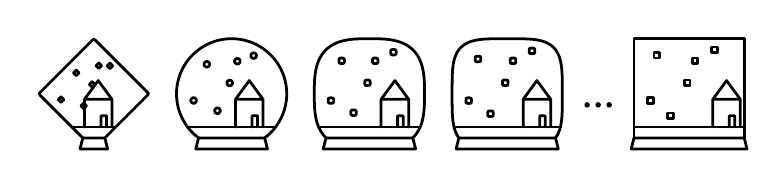
\begin{tikzpicture}[x=7mm,y=7mm,line cap=round,line join=round,line width=1pt]
\newcommand{\snowglobe}[1]{
\begin{scope}
\clip (-1.2,-0.8) rectangle (1.2,1.2);
\begin{scope}
\clip plot[samples=200,variable=\theta,domain=-90:270,smooth] ({cos(\theta) / (abs(sin(\theta))^#1+abs(cos(\theta))^#1)^(1/#1)},{sin(\theta) / (abs(sin(\theta))^#1+abs(cos(\theta))^#1)^(1/#1)});
\draw (-1,-0.6) -- (1,-0.6) ;
\draw[shift={({(0.68^#1-0.6^#1)^(1/#1)},-0.6)}] (-0.25,0) -- (-0.25,0.5) -- (0.25,0.5) -- (0.25,0) (0.25,0.5) -- (0,0.84) -- (-0.25,0.5) (0.05,0) -- (0.05,0.2) -- (0.15,0.2) -- (0.15,0);
\foreach \r/\theta in {0.6/80,0.4/230,0.7/190,0.2/100,0.8/60,0.7/130}
    \draw[shift={({\r*cos(\theta) / (abs(sin(\theta))^#1+abs(cos(\theta))^#1)^(1/#1)},{\r*sin(\theta) / (abs(sin(\theta))^#1+abs(cos(\theta))^#1)^(1/#1)})},scale=0.05]
        plot[samples=100,variable=\theta,domain=-90:270,smooth] ({cos(\theta) / (abs(sin(\theta))^#1+abs(cos(\theta))^#1)^(1/#1)},{sin(\theta) / (abs(sin(\theta))^#1+abs(cos(\theta))^#1)^(1/#1)});
\end{scope}
\draw plot[samples=200,variable=\theta,domain=-90:270,smooth] ({cos(\theta) / (abs(sin(\theta))^#1+abs(cos(\theta))^#1)^(1/#1)},{sin(\theta) / (abs(sin(\theta))^#1+abs(cos(\theta))^#1)^(1/#1)});
\end{scope}
\draw ({(1-0.8^#1)^(1/#1)},-0.8) -- ({(1-0.8^#1)^(1/#1)+0.05},-1) -- ({-(1-0.8^#1)^(1/#1)-0.05},-1) -- ({-(1-0.8^#1)^(1/#1)},-0.8) -- cycle;
}
\begin{scope}[shift={(0,0)}]
\snowglobe{1}
\end{scope}
\begin{scope}[shift={(2.5,0)}]
\snowglobe{2}
\end{scope}
\begin{scope}[shift={(5,0)}]
\snowglobe{3}
\end{scope}
\begin{scope}[shift={(7.5,0)}]
\snowglobe{4}
\end{scope}
\begin{scope}[shift={(9.15,0)}]
\fill (-0.2,-0.2) circle (0.05);
\fill (0,-0.2) circle (0.05);
\fill (0.2,-0.2) circle (0.05);
\end{scope}

\begin{scope}[shift={(10.8,0)}]
\begin{scope}
\clip (-1.2,-0.8) rectangle (1.2,1.2);
\begin{scope}
\clip (-1,-1) rectangle (1,1);
\draw (-1,-0.6) -- (1,-0.6) ;
\draw[shift={(0.68,-0.6)}] (-0.25,0) -- (-0.25,0.5) -- (0.25,0.5) -- (0.25,0) (0.25,0.5) -- (0,0.84) -- (-0.25,0.5) (0.05,0) -- (0.05,0.2) -- (0.15,0.2) -- (0.15,0);
\foreach \r/\theta in {0.6/80,0.4/230,0.7/190,0.2/100,0.8/60,0.7/130}
    \draw[shift={({\r*cos(\theta) / max(abs(sin(\theta)),abs(cos(\theta)))},{\r*sin(\theta) / max(abs(sin(\theta)),abs(cos(\theta)))})},scale=0.05]
        (-1,-1) rectangle (1,1);
\end{scope}
\draw (-1,-1) rectangle (1,1);
\end{scope}
\draw (1,-0.8) -- (1.05,-1) -- (-1.05,-1) -- (-1,-0.8) -- cycle;
\end{scope}
\end{tikzpicture}
\end{center}
\vspace{1mm}
\end{minipage}


\end{document}

